\documentclass[manuscript,review,anonymous]{acmart}

\usepackage{booktabs}
\usepackage{tabularx}
\usepackage{graphicx}
\graphicspath{{figures/pdf/}}

\settopmatter{printacmref=true,printccs=true,printfolios=true}
\setcopyright{none}
\acmConference[CHI '27]{Proceedings of the 2027 CHI Conference on Human Factors in Computing Systems}{May 2027}{Barcelona, Spain}
\acmYear{2027}
\copyrightyear{2027}

\newcommand{\term}[1]{\textbf{#1}}
\newcommand{\condition}[1]{\textsf{#1}}
\newcolumntype{Y}{>{\raggedright\arraybackslash}X}

\title{Evaluating Cross-Layer Integrity in Updates to Generated Clinical Interfaces}
\author{Anonymous Author(s)}

\begin{document}

\begin{abstract}
Generated clinical interfaces must do more than produce executable SQL and renderable screens: they must deliver the patient, item, time range, source, and presentation required by a clinical scenario. We define a cross-layer inconsistency as a broken correspondence among an information need, SQL, its result, and its presentation. Using EHRSQL-2024 and MIMIC-IV Demo, we deterministically generated eight inconsistency types and compared local validation, per-artifact contracts, a graph contract linking request to presentation, and a flat contract containing the same relations. Across 6,104 validations from 763 update pairs, local validation and per-artifact contracts accepted 100.00\% and 48.10\% of inconsistent candidates. Graph and flat contracts rejected every inconsistent candidate and accepted every valid one. Their identical results show that executable cross-layer relations, rather than graph storage itself, enabled detection. We position integrity as a prerequisite for evaluating clinically appropriate user experiences, not as evidence of user benefit.
\end{abstract}

\begin{CCSXML}
<ccs2012>
  <concept>
    <concept_id>10003120.10003121</concept_id>
    <concept_desc>Human-centered computing~Human computer interaction (HCI)</concept_desc>
    <concept_significance>500</concept_significance>
  </concept>
  <concept>
    <concept_id>10003120.10003123.10011760</concept_id>
    <concept_desc>Human-centered computing~Interactive systems and tools</concept_desc>
    <concept_significance>300</concept_significance>
  </concept>
</ccs2012>
\end{CCSXML}

\ccsdesc[500]{Human-centered computing~Human computer interaction (HCI)}
\ccsdesc[300]{Human-centered computing~Interactive systems and tools}

\keywords{generative user interfaces, data-driven interfaces, electronic health records, integrity validation, incremental updates, traceability}

\maketitle

\section{Introduction}

A useful clinical interface depends on the situation in which it is used. In a preoperative anesthesia clinic, a clinician may need to assemble a patient's background, planned procedure, and recent tests for a one-time assessment and then document anesthesia risks. In follow-up after thyroid surgery, a clinician may instead compare thyroid function, ultrasound findings, and hormone-replacement doses every three to six months. The same electronic health record therefore calls for different variables, time windows, sources, and presentations. The goal of a generated interface is not merely to produce SQL. It is to return the information required for a clinical task in a form that a clinician can review.

Existing technical checks leave a gap relative to that goal. SQL syntax, query execution, result schemas, interface code, and rendering can each be validated independently. Yet every artifact may pass while a query selects another patient, omits a time filter, leaves a result from the previous update, or connects a widget to the wrong data. Better text-to-SQL accuracy does not ensure that the same information need survives subsequent execution, connection, and presentation. A system can therefore work mechanically while returning information that does not answer the user's request.

We call a broken semantic correspondence between a scenario-grounded information need and the displayed information a \term{cross-layer inconsistency}. We evaluate a generated clinical interface as a process spanning an information need, SQL, an execution result, and a presentation, rather than as a collection of independently valid artifacts. Correctness here does not mean that the complete clinical judgment is correct. It means that the patient, item, time, aggregation, source, presentation, connection, and version specified for an update remain consistent across layers.

Research on generative and malleable interfaces has connected natural-language requests to interfaces through task models and semantic representations. Jelly preserves evolving information tasks in a task-driven data model and supports updates through natural language and direct manipulation~\cite{cao2025jelly}. Bridging Gulfs places a semantic representation of design intent between user input and generated interfaces so that users can inspect interpretations as they generate~\cite{park2026bridging}. SimStep separates concept, scenario, learning-objective, and interface graphs, allowing people to inspect and repair assumptions at multiple levels~\cite{kaputa2026simstep}. These systems demonstrate the value of intermediate representations. They do not, however, compare which relationships fail across a data-backed interface update and which validation conditions detect those failures on the same candidates.

We built an evaluation framework for cross-layer inconsistencies in generated clinical interface updates. We execute the clinical information requests and reference SQL in EHRSQL-2024~\cite{lee2024ehrsql} on the publicly available MIMIC-IV Clinical Database Demo v2.2~\cite{johnson2023mimic} and construct baseline data-driven interfaces. We then introduce one of eight inconsistencies: patient, clinical item, time, aggregation, information source, presentation, data-presentation connection, or stale result. An oracle implemented independently from candidate generation verifies the expected labels. Each candidate is evaluated under the same four validation conditions. This benchmark measures one prerequisite in the process of generating a clinically appropriate user experience: whether the requested information reaches the presentation unchanged.

We ask:

\begin{description}
  \item[RQ1] What information errors pass when SQL and presentation components are validated individually?
  \item[RQ2] How do local validation, per-artifact contracts, and contracts spanning request to presentation differ in inconsistency leakage, valid-update acceptance, and fault localization?
  \item[RQ3] Which inconsistencies can be corrected by one automatic repair based on a localized validation failure?
\end{description}

After freezing the evaluation method, we ran the test split once. We formed 763 update pairs from 134 question templates and performed 6,104 validations of valid and inconsistent candidates under four conditions. Local validation accepted all 763 inconsistent candidates, while per-artifact contracts accepted 367. A graph contract linking the question to the presentation and a flat contract storing the same relations both rejected every inconsistent candidate and accepted every valid candidate. They produced identical decisions, localizations, and one-step repairs. This result does not support an advantage of graph storage for detection. What separated the conditions was the ability to represent cross-layer semantic relations as executable contracts.

This paper makes five contributions:

\begin{itemize}
  \item We separate the evaluation of generated clinical interfaces into the clinical validity of task definitions, cross-layer integrity, and clinicians' use of the resulting presentation, recognizing that information needs and appropriate presentations vary by clinical scenario.
  \item We operationalize information errors in incremental data-driven interface updates as eight inconsistency types covering patient, item, time, aggregation, source, presentation, connection, and stale result.
  \item We provide a reproducible method that deterministically generates inconsistent candidates on public demo data and checks them with an oracle independent of candidate generation.
  \item We apply four validation conditions to the same candidates and quantify where artifact-level validity fails to ensure cross-layer integrity.
  \item From the null difference between graph and flat contracts with equivalent content, we derive the design implication that generated interfaces require testable cross-layer relations, not a particular storage format.
\end{itemize}

This is a technical evaluation. It does not evaluate the clinical validity of the scenario models, clinical safety, diagnostic accuracy, usability, cognitive load, clinical outcomes, or deployment. We maintain this boundary while arguing that the integrity of retrieval and presentation is a prerequisite for returning value to users.

\section{Related Work}

\subsection{Generative and Malleable User Interfaces}

Generative-interface research has moved from producing screens from natural language or examples toward helping users understand, edit, and reuse generated artifacts. DirectGPT supports iterative work with large language models by combining conversation with direct manipulation and reference resolution on generated objects~\cite{masson2024directgpt}. DynaVis combines conversational generation and editing of visualizations with direct interaction on the generated interface~\cite{vaithilingam2024dynavis}. Both treat generated artifacts as objects that continue to change, rather than as one-shot outputs.

Intermediate representations provide structure for such updates. Jelly places a task-driven data model behind a generated interface and propagates task changes into data and views~\cite{cao2025jelly}. Bridging Gulfs uses semantic representations to narrow gaps among user intent, model interpretation, and interface output~\cite{park2026bridging}. SimStep separates graphs for concepts, scenarios, learning objectives, and interfaces so that assumptions can be inspected and repaired across stages~\cite{kaputa2026simstep}. Across these systems, intermediate representations become points of contact for inspection and repair.

We study a narrower question. We do not compare initial generation quality or the experience of editing an interface. We test whether semantic relations to data survive an update. Although our system can store relations as a graph, the graph form is not itself a claimed contribution. We also encode equivalent relations in a flat representation, separating the effect of validation content from the effect of storage form.

\subsection{Inspection and Repair in Human-AI Collaboration}

People do not simply accept or reject generated suggestions. Ignore, Trust, or Negotiate documents how clinicians ignore, trust, and negotiate AI suggestions, and argues for interactions that expose uncertainty and supporting information~\cite{sivaraman2023ignore}. For generated interfaces, an undifferentiated error message may be less actionable than a diagnosis that identifies the broken relationship and the scope affected by a repair.

Debugging support must enable movement from detecting failure to locating its cause. We measure detection, fault localization, and one-step repair separately. This distinction separates a validator that rejects broadly from one that returns a diagnosis that can drive correction. We do not evaluate whether a person understands the resulting diagnosis. Machine-readable localization and support for human judgment remain separate research questions.

\subsection{From Natural-Language Questions to Data and Presentation}

Text-to-SQL research evaluates whether a system can generate executable SQL that answers a natural-language question. EHRSQL-2024 provides a shared task for electronic health records that includes both answerable and unanswerable questions~\cite{lee2024ehrsql}. Its central challenges include generating SQL for answerable questions and abstaining when a question cannot be answered.

We do not compare SQL-generation performance. We use reference SQL as a starting point and examine inconsistencies that arise during subsequent updates. Even when a correct query was previously available, a question, query, result, or presentation can advance to a different version during an update. An executable query can also refer to a patient or time range that differs from the request. Validation must therefore cover not only question-to-SQL correspondence, but also SQL-to-result versioning, result-to-presentation compatibility, data-presentation connections, and update versions.

\subsection{Model Transformation and Consistency}

Bidirectional-transformation research has formalized how updates to structured sources and views should correspond. Lenses define laws for transformations between a source and its view~\cite{foster2007lenses}. Metamorphic testing has also been proposed for model transformations where enumerating every correct output is difficult, using invariant relations instead of complete expected outputs~\cite{he2018metamorphic}.

We likewise avoid requiring exact equality of complete interface JSON. We encode the relationships that should change and those that should remain invariant. Stable identifiers, order, and display wording may vary without changing meaning, while a visually similar interface can still be inconsistent if it refers to another patient, a different period, or a stale result. Our contribution relative to prior consistency work is to place a user's natural-language information need, data retrieval, execution result, and presentation boundaries in one evaluation unit for generated-interface updates.

\section{Clinical Problem and Evaluation Scope}

\subsection{Scenario-Specific Information Needs}

Our design process organized two clinical scenarios that motivated this work: a preoperative anesthesia clinic and follow-up after thyroid surgery. In the preoperative scenario, the surgery date anchors a one-time assessment that brings together patient demographics, the planned procedure, lifestyle and allergy information, medical and treatment histories, recent examinations, and prior anesthesia records. The clinician ultimately compiles a list of anesthesia risks. This scenario emphasizes a broad view of the patient's latest state.

In post-thyroidectomy follow-up, the visit date anchors the review. The clinician examines thyroid function, ultrasound findings, and levothyroxine replacement dose. Thyroid function and dose require a twelve-month trend, while other tasks use the latest values. Appropriate views therefore combine longitudinal trends with current summaries.

Figure~\ref{fig:scenario-to-value} illustrates these differences and the scope of this paper. The scenarios are design examples, not clinically validated ground truth for our benchmark. Their task models have not completed expert validation. We use them to explain why the information and presentation retrieved from the same electronic health record must depend on a clinical scenario.

\begin{figure}[t]
  \centering
  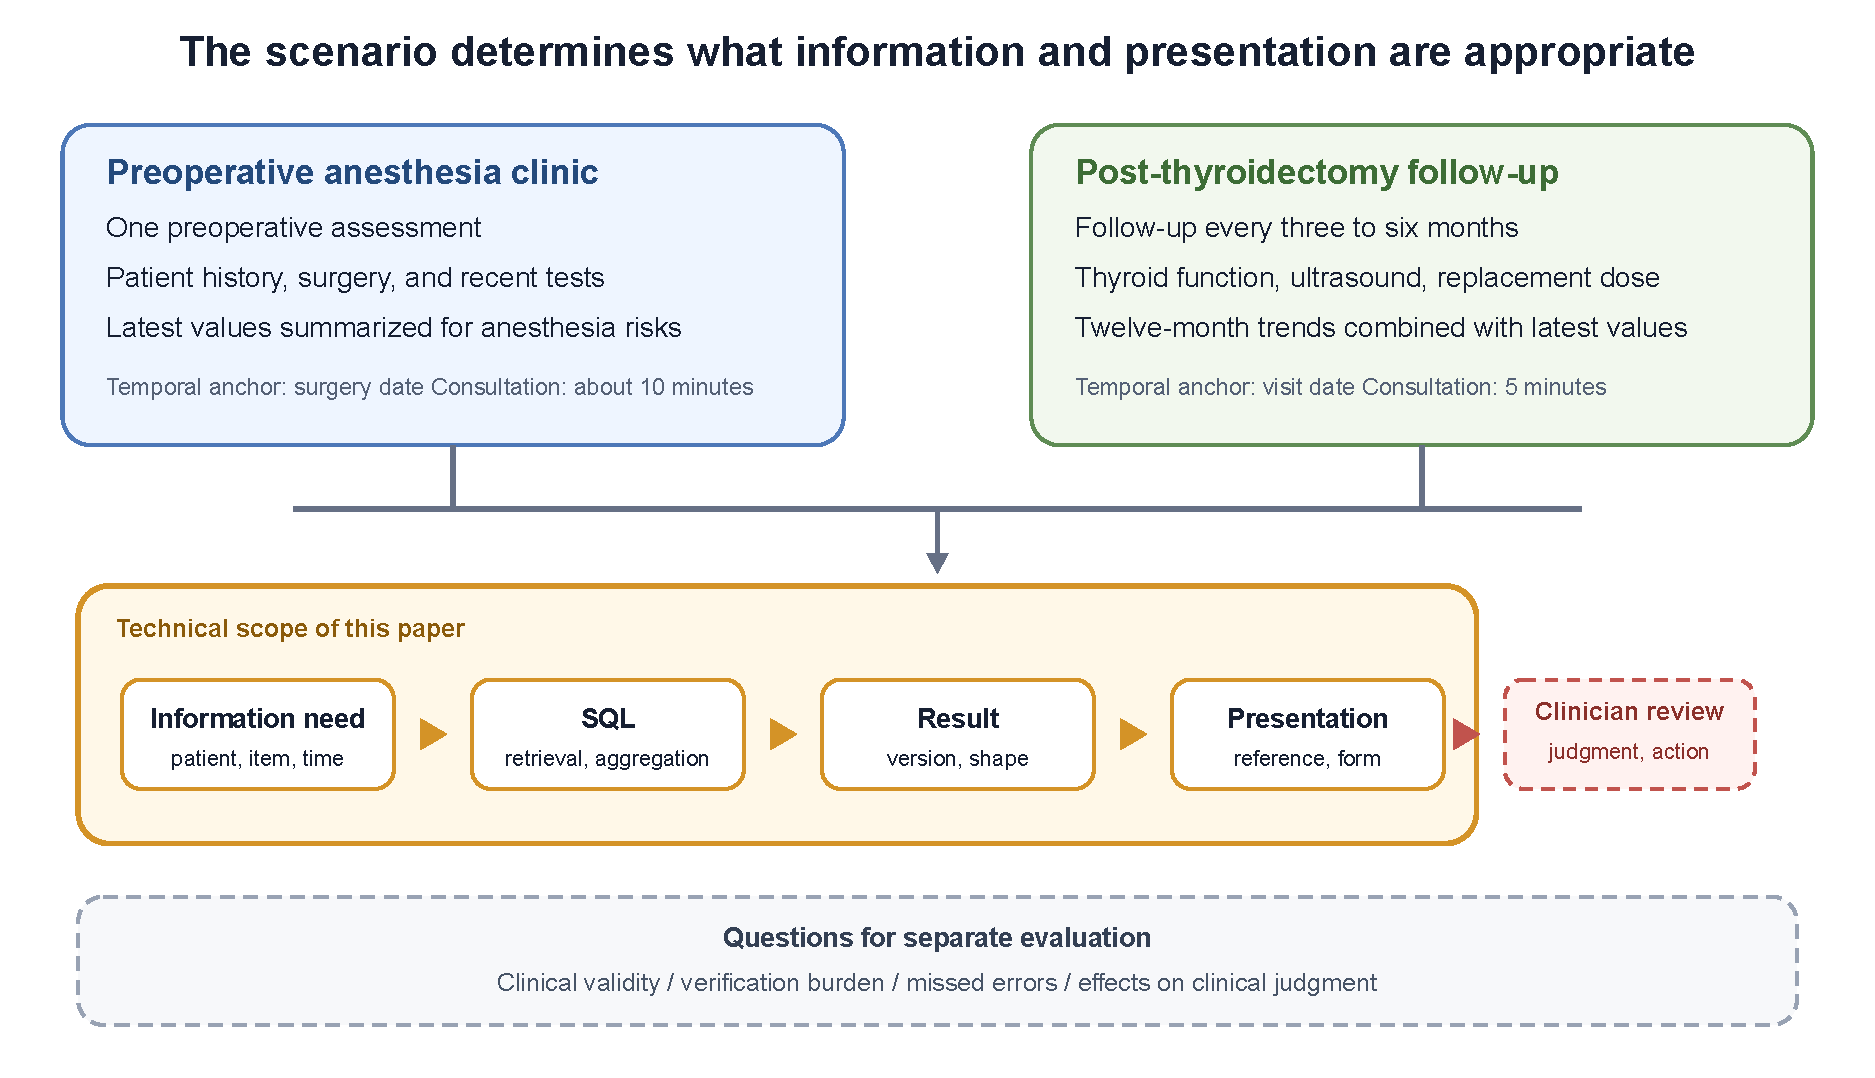
\includegraphics[width=\linewidth]{scenario-to-value-en.pdf}
  \caption{From clinical scenarios to user value, with the technical scope evaluated in this paper. The scenarios are design examples rather than formal benchmark cases.}
  \Description{The preoperative anesthesia clinic and post-thyroidectomy follow-up have different temporal anchors, information needs, and presentation forms. The technical evaluation covers the path from information need through SQL and execution result to presentation. Clinical review and judgment, clinical validity, verification burden, missed errors, and effects on judgment are marked for separate evaluation.}
  \label{fig:scenario-to-value}
\end{figure}

\subsection{A Causal Path to User Value}

At least three conditions separate a generated clinical interface from value to a clinician. First, domain experts must define questions, required information, and completion criteria for a clinical scenario. Second, the system must translate the resulting information need into appropriate retrieval and presentation. Third, a clinician must use the presentation to review necessary information and perform the clinical task. This paper directly evaluates the second condition.

Our results cannot show that cross-layer integrity reduces verification effort or missed information. Instead, integrity is a precondition for evaluating an experience built on appropriate information. Measuring completion time or preference on a screen that refers to the wrong patient or period would not establish that the interface supports its intended clinical task. A future study should use expert-reviewed scenarios and synthetic cases to measure incorrect acceptance of faulty updates, acceptance of valid updates, fault localization, repair, review time, interaction counts, and cognitive load as distinct outcomes.

\subsection{Defining an Information Error}

Information can be wrong at several stages. This study does not determine whether source records are factually correct, whether a scenario's task model is clinically appropriate, or whether a clinician makes the correct judgment after viewing the interface. We define an \term{information error} within our scope as a state in which information delivered to the screen does not match a specified information need in at least one of eight dimensions: patient, item, time, aggregation, source, presentation, connection, or version. A cross-layer inconsistency localizes such an error to a relationship between artifacts.

This definition distinguishes a query that fails to run from a query that runs while retrieving different information. Local validation can detect the former. Detecting the latter requires comparison between the information need and SQL, between SQL and its execution result, and between the result and its presentation.

\section{Defining Cross-Layer Integrity}

\subsection{Information Flow and Detection Mechanism}

We model four layers: information need, SQL, execution result, and presentation component. An information need includes the target patient, clinical item, time, aggregation, source, and expected presentation. SQL translates that need into a database operation. An execution result has a version corresponding to the SQL, input, and time of execution. A presentation component refers to a result and displays it using a form compatible with its shape.

\begin{figure}[t]
  \centering
  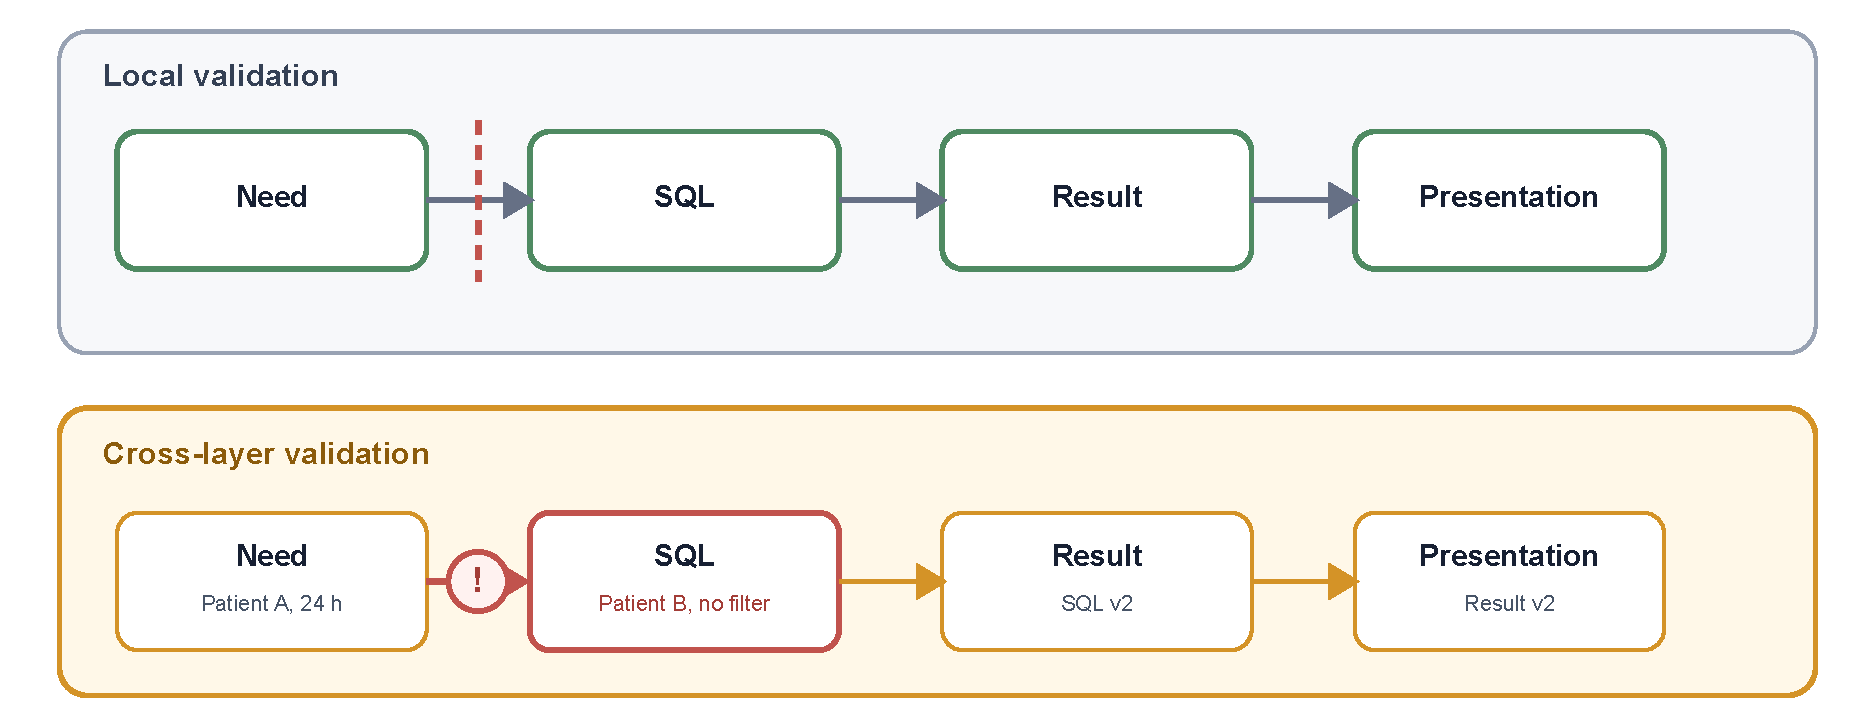
\includegraphics[width=\linewidth]{detection-mechanism-en.pdf}
  \caption{Local validation compared with a cross-layer contract. By comparing semantic keys and versions across adjacent layers, the contract detects information that is independently valid but inconsistent with the request.}
  \Description{The top row shows an information need, SQL, result, and presentation passing local checks, while a patient and time mismatch between the need and SQL is not checked. The bottom row shows Patient A and the last 24 hours in the information need but Patient B and no time filter in SQL. The patient and time predicates fail, localizing the fault between the request and SQL.}
  \label{fig:detection-mechanism}
\end{figure}

Figure~\ref{fig:detection-mechanism} explains why cross-layer inconsistencies are detectable. Local validation inspects only the inside of each box. A cross-layer contract compares semantic keys parsed from an information need against the parsed SQL; compares the SQL version against the result version; and compares the result reference and shape against the presentation component. On a mismatch, it returns both the failed predicate and the pair of artifacts joined by that predicate. Detection therefore does not arise from graph traversal alone. It arises because equivalent meanings can be compared at artifact boundaries.

An update candidate $c$ satisfies cross-layer integrity when the information need and SQL have the same meaning, the SQL and execution result have matching versions, and the result and presentation agree in reference and presentation form. We express this as:

\begin{equation}
I(c)=P(c)\land D(c)\land T(c)\land A(c)\land S(c)\land V(c)\land L(c)\land R(c)
\end{equation}

$P$ denotes patient, $D$ clinical item, $T$ time, $A$ aggregation, $S$ source, $V$ presentation form, $L$ the data-presentation link, and $R$ the correspondence between SQL and result versions. Valid candidates satisfy all eight predicates. Each inconsistent candidate violates exactly one.

\subsection{Eight Inconsistency Types}

Table~\ref{tab:mutations} defines the eight inconsistencies. A patient inconsistency preserves the patient in the information need while changing the patient condition in SQL to another valid candidate. An item inconsistency changes the selected column or aggregation target. A time inconsistency changes a condition associated with a time point or interval. An aggregation inconsistency replaces a count, maximum, minimum, average, or related operation with another valid operation.

\begin{table}[t]
  \caption{Eight cross-layer inconsistencies generated for evaluation}
  \label{tab:mutations}
  \begin{tabularx}{\linewidth}{lYY}
    \toprule
    Type & Mutated element & Checks the candidate may still pass \\
    \midrule
    Patient & Patient condition in SQL & Syntax, read-only, execution \\
    Clinical item & Selected column or target & Syntax, execution, result type \\
    Time & Point or interval condition & Syntax, execution \\
    Aggregation & Count, maximum, minimum, mean, etc. & Syntax, execution, result type \\
    Source & Referenced table & Syntax, execution \\
    Presentation & Component used to show result & UI structure, rendering \\
    Connection & Data node referenced by component & Per-node type \\
    Stale result & Result version after SQL update & SQL execution, result type, rendering \\
    \bottomrule
  \end{tabularx}
\end{table}

A source inconsistency changes the table referenced by SQL relative to the source associated with the information need. For presentation inconsistency, SQL, result, columns, and values remain fixed while the baseline component type changes: for example, a scalar metric becomes a dataframe, or a dataframe uses another table component. A connection inconsistency redirects a presentation component to another data node. A stale-result inconsistency updates SQL while retaining the execution result from the earlier version.

These categories are not an empirical distribution of errors observed in clinical practice. They form a fault model that makes specific relationships testable. Because we inject one inconsistency into each candidate, the results do not characterize performance on compound failures.

\section{Evaluation Framework}

\subsection{Constructing Baseline Cases}

The inputs are answerable questions and reference SQL from EHRSQL-2024. Unanswerable cases lack reference SQL from which to construct a baseline interface, so we exclude them from the primary evaluation while recording their count. Reference queries are executed read-only against the SQLite version of MIMIC-IV Demo v2.2. We reject statements that write data, contain multiple statements, or use disallowed syntax before execution, and impose a five-second limit on each query.

We use a metric component when an execution result is a single value and a dataframe when it contains multiple rows or columns. Empty results are retained as results with a defined column structure. Each baseline case stores semantic slots parsed from the question template, parsed SQL, result shape, data node, presentation component, and version identifiers for these artifacts.

Cases sharing a question template and SQL structure are paired as before-and-after updates. From each pair, we create a valid candidate in which all relations are updated together and an inconsistent candidate in which exactly one relation is broken. Candidates derived from the same question form are not independent. Our statistical procedure therefore resamples question templates rather than individual candidates.

\subsection{Independent Oracle}

Candidate generation and ground-truth evaluation are implemented as separate processes. The oracle compares semantic slots from the question template, parsed SQL, the execution result's shape and version, and references between data nodes and presentation components. Evaluation stops if the label expected by the candidate generator disagrees with the oracle.

The oracle does not require exact equality of complete JSON. This choice permits differences in stable identifiers, ordering, and presentation text that do not change meaning. Conversely, a candidate is inconsistent when it refers to another patient, period, or result version even if the visible screen appears similar. The oracle thereby separates surface similarity from semantic correspondence.

\subsection{Four Validation Conditions}

We apply the same candidate to the four conditions in Table~\ref{tab:conditions}. \condition{Local validation} checks artifacts separately: SQL must be read-only and executable, artifacts must conform to their schemas, and the presentation component must accept the result type. \condition{Artifact contracts} add conditions within SQL, result, and presentation artifacts, but do not maintain one relationship spanning the information need to presentation.

The \condition{graph contract} represents question templates, SQL, results, data nodes, and presentation components as nodes, with edges for patient, item, time, aggregation, source, version, reference, and presentation relations. After an update, affected relations are evaluated again. The \condition{flat contract} stores the same semantic slots and correspondences in a single sidecar table and validates the same predicates. Giving both conditions equivalent content separates the effect of what is checked from the effect of graph storage.

\begin{table}[t]
  \caption{Four validation conditions}
  \label{tab:conditions}
  \begin{tabularx}{\linewidth}{lYYY}
    \toprule
    Condition & Individual artifacts & Cross-layer relations & Storage \\
    \midrule
    Local validation & Basic checks & None & Artifacts \\
    Artifact contracts & Detailed checks & Partial & Artifacts \\
    Graph contract & Detailed checks & All & Nodes and edges \\
    Flat contract & Detailed checks & All & One table \\
    \bottomrule
  \end{tabularx}
\end{table}

\subsection{Localization and One-Step Repair}

When a validator rejects a candidate, it returns the failed predicate and the related artifacts as a diagnosis. We count localization as successful only when the diagnosis identifies the injected inconsistency type. Detecting an inconsistency while returning the wrong location or type does not count as successful localization.

Repair uses the diagnosis once to restore a value uniquely determined by the baseline contract. A presentation component's reference, result version, or presentation form can, for example, be restored from its correspondence in the contract. We run the oracle's integrity predicates after repair and count success only if the candidate satisfies all of them. Repair does not search, retry, or invoke a generative model.

\subsection{Evaluation Protocol}

Figure~\ref{fig:protocol} summarizes the protocol. On development data, we prioritized 50 cases with distinct question templates to verify SQL execution and baseline conversion. On validation data, we checked candidate counts per inconsistency type, the number of represented templates, label agreement, and the requirement that saved outputs contain no sensitive data. A planned column-order mutation could not be generated, so before inspecting the test split we replaced it with the presentation mutation. We left all other mutations, metrics, analyses, and stopping rules unchanged.

\begin{figure}[t]
  \centering
  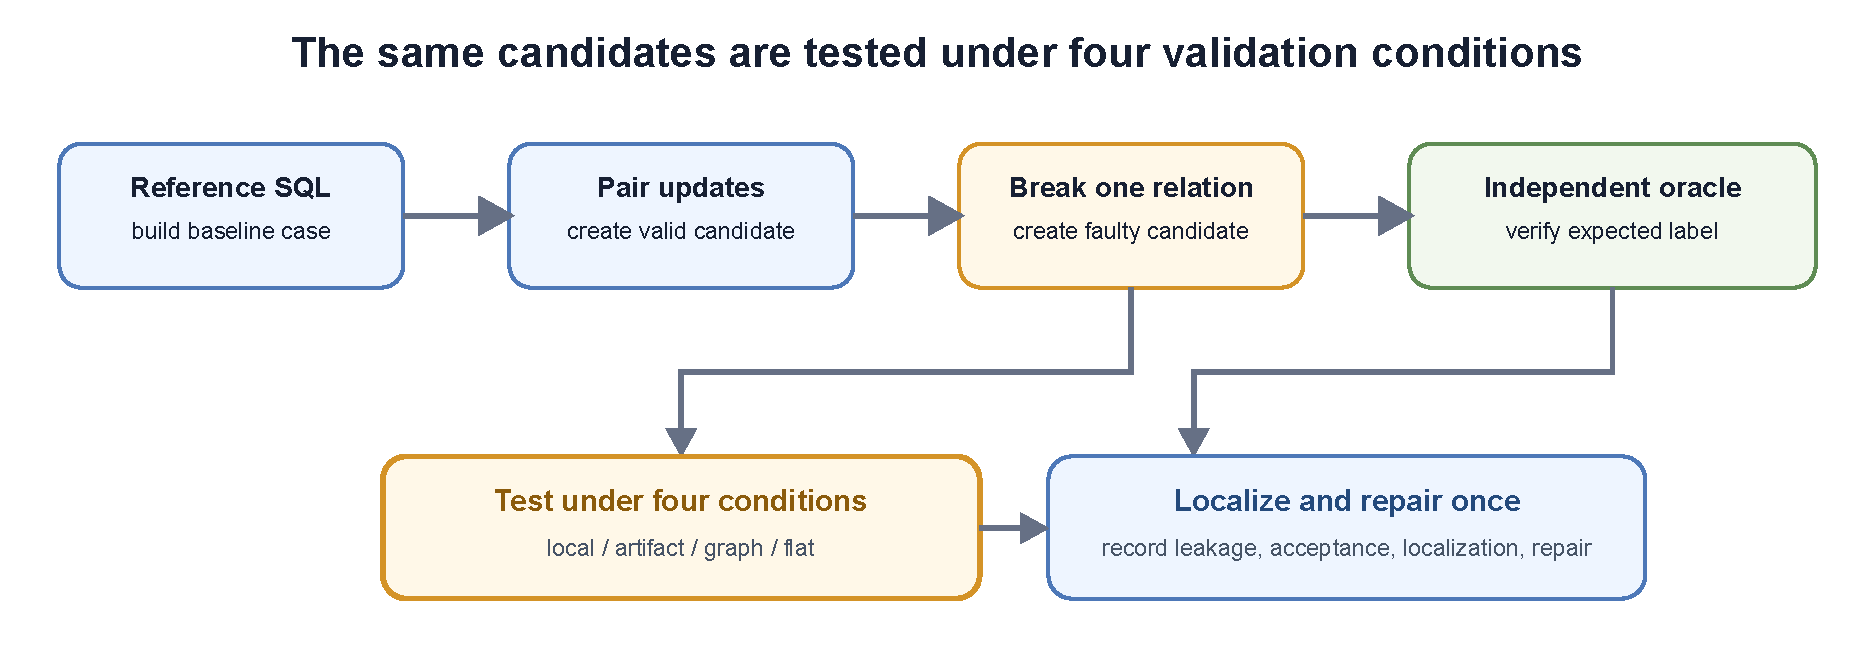
\includegraphics[width=\linewidth]{evaluation-protocol-en.pdf}
  \caption{Evaluation protocol from baseline construction through candidate generation, validation, localization, and repair.}
  \Description{Reference SQL produces a baseline case. Before-and-after cases form a valid candidate, and one relation is broken to form an inconsistent candidate. An independent oracle verifies labels. The same candidates are evaluated under four conditions, followed by localization and one repair attempt.}
  \label{fig:protocol}
\end{figure}

After the validation-data criteria were met, we froze the evaluation code, configuration, and analysis at Git commit \texttt{baa82075b6bf}. We then ran the test split once. No generative or external model was called during evaluation.

\subsection{Metrics and Statistical Analysis}

The primary metrics are \term{inconsistency leakage rate} and \term{valid-update acceptance rate}. Leakage is the proportion of injected inconsistent candidates accepted by a validator and is better when lower. Valid acceptance is the proportion of candidates with all relations correctly updated that are accepted and is better when higher. Secondary metrics are fault-localization rate, one-step repair success rate, and mean validation time per candidate.

We calculate condition differences within the same candidates. We obtain 95\% confidence intervals from 10,000 cluster bootstrap resamples at the question-template level. Resampling templates rather than candidates prevents cases derived from the same SQL structure and mutation rule from being treated as independent examples.

\subsection{Data Management and Reproducibility}

Released artifacts do not contain raw data, question text, reference SQL, patient identifiers, or patient-level result values. They contain hashed case identifiers, input and candidate checksums, inconsistency type, decision, diagnosis, repair outcome, aggregates, and execution environment. We froze formal results as JSON and JSON Lines, then converted them to TSV in an independent procedure that recomputed counts, primary metrics, and confidence intervals. The recomputed values matched the original summary.

\section{Results}

\subsection{Baseline Cases and Candidates}

The test split contained 1,167 cases. We evaluated the 934 answerable cases with reference SQL and excluded 233 unanswerable cases from the primary evaluation. Reference SQL executed and baseline artifacts were constructed successfully for all 934 cases; 82 yielded empty results with defined column structures. We formed 763 before-and-after update pairs from 134 question templates. For each pair, we created one valid and one inconsistent candidate and applied four conditions, yielding $763\times2\times4=6{,}104$ validations. Candidate labels disagreed with the independent oracle in zero cases.

We generated 52 patient, 55 item, 106 time, 34 aggregation, 134 source, 134 presentation, 129 connection, and 119 stale-result inconsistencies, totaling 763. For patient, item, time, and aggregation mutations, we skipped cases where no alternative SQL could change exactly one semantic dimension. Candidate counts therefore differ across types and depend on the data and question forms.

\subsection{RQ1: Inconsistencies That Pass Local Validation}

Local validation accepted every inconsistent candidate across all eight types, producing a leakage rate of 100.00\%. Each candidate was constructed to remain valid as read-only executable SQL and to have an independently valid result and presentation component. The result shows that individually checking syntax, schemas, and renderability does not detect patient or time errors, presentation errors, data-presentation misconnection, or stale results.

Leakage under artifact contracts varied by inconsistency type. As Table~\ref{tab:mutation-results} shows, artifact contracts rejected every source, presentation, and stale-result inconsistency. In contrast, 92.73\% to 98.08\% of patient, item, time, and aggregation inconsistencies leaked, as did every connection inconsistency. Conditions expressible inside an artifact were checked, but cross-artifact correspondences between the need and SQL or between a data node and presentation remained weak points.

\begin{table}[t]
  \caption{Artifact-contract leakage by inconsistency type}
  \label{tab:mutation-results}
  \begin{tabularx}{\linewidth}{Yrrr}
    \toprule
    Type & Generated & Leaked & Leakage rate \\
    \midrule
    Patient & 52 & 51 & 98.08\% \\
    Clinical item & 55 & 51 & 92.73\% \\
    Time & 106 & 103 & 97.17\% \\
    Aggregation & 34 & 33 & 97.06\% \\
    Source & 134 & 0 & 0.00\% \\
    Presentation & 134 & 0 & 0.00\% \\
    Connection & 129 & 129 & 100.00\% \\
    Stale result & 119 & 0 & 0.00\% \\
    \midrule
    Total & 763 & 367 & 48.10\% \\
    \bottomrule
  \end{tabularx}
\end{table}

\subsection{RQ2: Detection, Acceptance, and Localization}

Table~\ref{tab:main-results} presents the primary and secondary results. The graph and flat contracts rejected all 763 inconsistent candidates and accepted all 763 valid candidates. Compared with local validation, the leakage difference was $-100.00$ percentage points with a 95\% confidence interval of $[-100.00,-100.00]$. Compared with artifact contracts, it was $-48.10$ points, with a 95\% confidence interval of $[-49.56,-46.53]$. Valid-update acceptance was 100.00\% for all four conditions, yielding no condition difference.

\begin{table}[t]
  \caption{Primary and secondary results across four conditions}
  \label{tab:main-results}
  \begin{tabularx}{\linewidth}{Yrrrr}
    \toprule
    Condition & Leakage & Valid accepted & Localized & Mean time \\
    \midrule
    Local validation & 763/763 & 763/763 & 0/763 & 2.152 ms \\
    Artifact contracts & 367/763 & 763/763 & 387/763 & 7.441 ms \\
    Graph contract & 0/763 & 763/763 & 763/763 & 9.339 ms \\
    Flat contract & 0/763 & 763/763 & 763/763 & 9.296 ms \\
    \bottomrule
  \end{tabularx}
\end{table}

Artifact contracts correctly localized the injection in 387 of the 396 inconsistent candidates that they rejected, for an overall localization rate of 50.72\%. Graph and flat contracts localized the type and location in all 763 cases. The two full-relation conditions disagreed on zero decisions, and their difference in leakage was zero points. Mean validation time per candidate was 2.152 ms for local validation, 7.441 ms for artifact contracts, 9.339 ms for the graph contract, and 9.296 ms for the flat contract. In this implementation and environment, the difference between the two full-relation conditions was 0.043 ms.

\subsection{RQ3: One-Step Repair}

Local validation did not detect inconsistent candidates and therefore attempted no repair. Artifact contracts attempted one repair on each of the 396 candidates they rejected, after which 387 satisfied every predicate of the independent oracle. The repair success rate among attempted cases was 97.73\%. Nine remained inconsistent after the single repair.

Graph and flat contracts localized all 763 inconsistent candidates, and all 763 satisfied every integrity predicate after one repair. Neither condition rejected a valid candidate, and no repair was applied to valid candidates. This 100\% result is bounded by our use of one known fault, a known contract, and a deterministic repair rule. It does not generalize to compound or naturally occurring generation errors.

\section{Discussion}

\subsection{From Correct SQL to a Correct Process for Generating UX}

All eight inconsistency types passed local validation. SQL, results, and presentation components must each work, but their independent operation does not ensure that a clinician receives the requested information. The appropriate unit of evaluation is therefore the process that begins with a clinical scenario, specifies an information need, retrieves data, and presents the result, rather than the query or screen alone.

Within this framing, improvement in SQL generation is one component of a longer process. A previously correct query can be followed by an incremental update that misaligns patient, time window, result version, or presentation target. The final screen then fails to answer the request. Conversely, a visually polished screen cannot be judged appropriate if its data source and provenance are unavailable for inspection. Generative-interface research should distinguish surface quality, artifact executability, information provenance, and user verification, and reconnect these evaluations to the same clinical task.

\subsection{Why Cross-Layer Contracts Detected the Errors}

Artifact contracts rejected all source, presentation, and stale-result inconsistencies but missed most patient, item, time, and aggregation inconsistencies and all connection inconsistencies. The former can be constrained within a single artifact through an allowlist, result shape, or version. The latter require a comparison between the request and query or between a data node and presentation component.

Cross-layer contracts retained patient, item, time, aggregation, source, and presentation as semantic keys and compared them between adjacent artifacts together with versions and references. They did not merely execute SQL again; they determined whether a value inherited from the request remained equivalent across an artifact boundary. Associating a failed predicate with the relation it checked enabled both localization and repair. This mechanism is necessary for interpreting a leakage rate of zero: the result came from explicitly testable correspondences, not from the storage structure alone.

\subsection{Clinical Scenarios Expose Domain-Specific Requirements}

The contrast between preoperative assessment and post-thyroidectomy follow-up explains why a clinical interface rarely has one universally correct view. A preoperative clinic assembles broad patient context and recent tests for one assessment. Thyroid follow-up repeatedly compares a narrower set of examinations and medications over time. The latest value may be appropriate in one task and a longitudinal trend in another, while the temporal anchor may be a surgery date or a visit date. Appropriate presentation follows from the scenario and task.

In medicine, whether information is displayed is insufficient: whose information it is, what it measures, when it was recorded, and where it came from can affect the evidence available for judgment. Showing another patient's data, an inappropriate time window, or a stale result cannot be treated as a minor rendering defect. A generated interface must connect expert-defined information needs, safety-relevant information, and task-completion criteria to provenance and update time. Our benchmark does not establish the clinical validity of the two scenarios or show that cross-layer contracts reduce clinical errors. The scenarios make design requirements concrete and identify what a subsequent expert evaluation must establish.

\subsection{Relational Content, Not Graph Storage, Produced the Result}

Graph and flat contracts produced identical decisions, localizations, and one-step repairs. The detection result supports only the claim that explicitly storing and checking the eight relationships allowed either representation to reject the tested candidates. Graph storage by itself cannot serve as evidence of safety or better performance.

This null result separates the storage representation from the capability presented to users. A graph may support impact exploration, propagation of partial updates, or visualization of relations, but our benchmark did not measure editing efficiency or comprehensibility. A future comparison should give both conditions the same atomic information and repair actions, then test whether presenting cross-layer paths as a graph helps clinicians locate and repair problems.

Jelly, Bridging Gulfs, and SimStep use intermediate representations as points at which users can inspect intent and edit generated artifacts~\cite{cao2025jelly,park2026bridging,kaputa2026simstep}. Our result adds a requirement for those contact points in data-backed systems: the represented relations should remain testable through execution results and presentation. The value of an intermediate representation depends not only on its structure, but on which relations connect user verification to system execution.

\subsection{Connecting Detection to User Value}

Successful machine detection is not itself a user benefit. Our results directly show that known single inconsistencies could be stopped before presentation and returned as machine-readable locations. To return that capability to clinicians, a system should include the diagnosis in the update interaction and allow users to accept, reject, or partially repair a proposed update.

A diagnosis such as ``the patient in the request does not match the patient condition in SQL'' or ``the presentation refers to a result from the previous version'' may narrow what a user must inspect compared with a generic ``invalid interface'' message. Whether diagnosis reduces review time, reduces acceptance of faulty updates, or instead causes excessive rejection of valid updates requires a human-participant comparison. Such a study could compare a final-screen-only condition against the same screen with cross-layer paths and diagnoses, reporting incorrect acceptance, valid acceptance, fault localization, semantically correct repair, time, and cognitive load separately.

Work on how clinicians ignore, trust, or negotiate generated suggestions~\cite{sivaraman2023ignore} also cautions against combining all decisions into one accuracy measure. A study should mix faulty and valid updates and report incorrect acceptance of faulty updates separately from acceptance of valid updates. This distinction reveals whether cross-layer information improves discrimination or merely increases a tendency to reject.

\subsection{Separating Automatic Repair from Human Judgment}

The two full-relation conditions repaired all 763 known single faults in one step. When a contract uniquely specifies a patient condition, reference, result version, or presentation form, the system can mechanically restore a minimal difference. Validation can therefore produce a repair candidate rather than ending with rejection.

An ambiguous natural-language request, a choice of clinically appropriate presentation granularity, or simultaneous changes to several artifacts may not have a unique repair. Generated interfaces should distinguish relations that can be repaired mechanically, relations that require presenting alternatives, and relations that require domain-expert judgment. The 100\% repair result does not demonstrate the general safety of automatic repair. It characterizes the bounded case in which a known contract identifies one value to restore.

\subsection{Transfer to Other High-Accuracy Domains}

Systems that retrieve data from an information need and generate a dashboard, table, or visualization can also arise in finance, aviation, and industrial operations. In these domains, an executable query and renderable screen likewise do not guarantee agreement in entity, period, source, or version. The structure of a cross-layer contract may therefore transfer.

The transferable element is the validation pattern, not the eight healthcare-oriented categories unchanged. Each domain must specify who makes which judgment, how incorrect information affects the task, which relations can be checked mechanically, and where responsibility passes to a person. Our HCI contribution is to add traceability and diagnosis from a user's task to the final presentation to evaluations of generated artifacts.

\section{Limitations and Ethics}

First, we inject one inconsistency at a time using deterministic rules. The generated candidates do not represent the distribution of errors that a generative model produces naturally. A condition that achieved 100\% on single faults may not perform similarly on compound failures, ambiguous requests, or unknown presentation components. Future work should apply the frozen validators to naturally occurring candidates and qualitatively analyze failures outside the taxonomy.

Second, the benchmark begins with reference SQL and therefore excludes initial errors from a text-to-SQL model. Question interpretation and query generation can fail in practice. Our result is limited to incremental updates after a valid reference is available. Evaluation that includes initial SQL generation must separately address abstention, multiple interpretations, and the clinical appropriateness of a query.

Third, we use only MIMIC-IV Demo v2.2 and EHRSQL-2024 question templates. The preoperative anesthesia and post-thyroidectomy scenarios illustrate the problem but are not formal evaluation cases. Candidate counts differ across inconsistency types because result shapes and valid alternatives differ. We cannot generalize the findings to other clinical scenarios, data models, institutions, complex visualizations, or updates spanning multiple sources.

Fourth, we intentionally give the graph and flat contracts equivalent relational content to isolate storage form. This comparison does not test editing at scale, implementation maintainability, or the understandability of explanations. Validation times come from one implementation and environment and should not be interpreted as general performance differences between representations.

Fifth, this is a technical evaluation on publicly available deidentified demo data. Reference SQL is a technical baseline, not a clinically validated definition of appropriate presentation. We did not measure effects on verification burden, acceptance of faulty updates, or clinical judgment. We make no claims about clinical safety, diagnostic accuracy, usability, cognitive load, clinical outcomes, deployment, or generalization across institutions. Any human-participant study will be separate work conducted only after applicable ethics review, permission, recruitment, consent, withdrawal, and data-management procedures are established.

Released artifacts contain no question text, reference SQL, patient identifiers, or patient-level result values. We state the conditions of use and provenance for MIMIC-IV Demo and EHRSQL-2024 and include only releaseable checksums, categories, decisions, and aggregate statistics in reproducibility materials.

\section{Conclusion}

Generating an interface appropriate for a clinical scenario requires more than retrieving data with executable SQL. The requested information must remain consistent through execution and presentation. We operationalized failures in that process as eight cross-layer inconsistencies, generated them deterministically on public demo data, and compared four validation conditions on the same candidates.

Across 763 update pairs and 6,104 validations, local validation accepted every inconsistency and artifact contracts accepted 48.10\%. Graph and flat contracts with equivalent content rejected every inconsistent candidate and accepted every valid one. Their identical results indicate that detection was supported by executable relations over patient, item, time, aggregation, source, presentation, connection, and version, rather than by graph storage itself.

A generated interface that will continue to change should be evaluated not only for its visible output and artifact-level validity, but also for provenance from a scenario-grounded information need to presentation and for diagnoses that explain failures. This study identifies a technical prerequisite and its detection mechanism before evaluating a clinically appropriate user experience. The next step is to apply it to expert-reviewed scenarios and test, with human participants, how cross-layer diagnoses affect acceptance of faulty updates, fault localization, repair, and verification burden.

\bibliographystyle{ACM-Reference-Format}
\bibliography{references}

\end{document}
